\documentclass{standalone}
\usepackage{tikz}
\usetikzlibrary{patterns, positioning}

\begin{document}
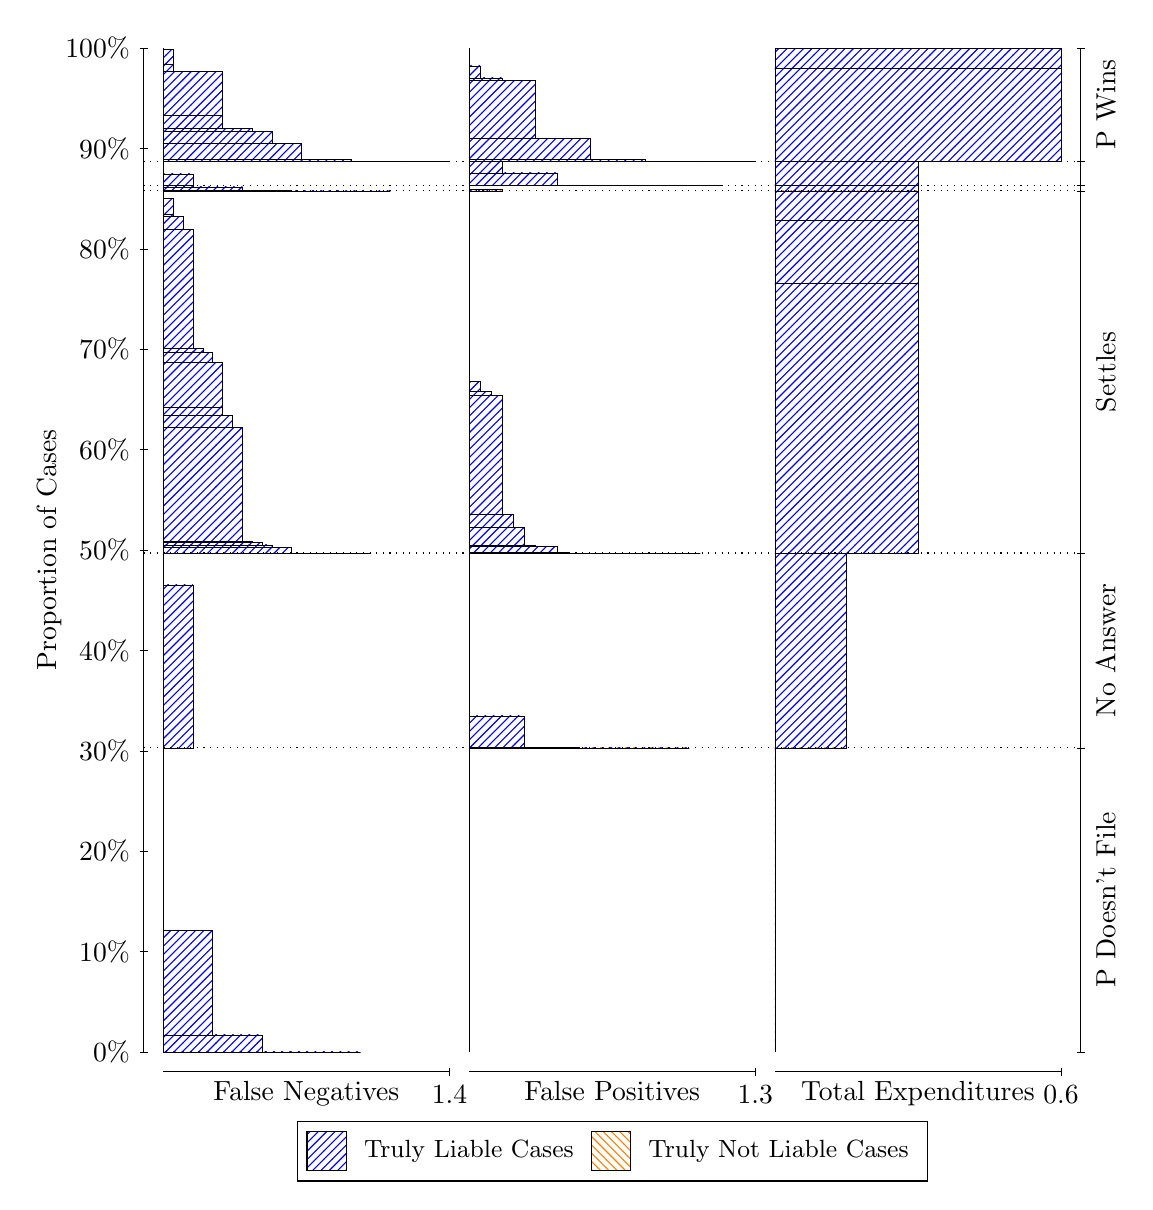
\begin{tikzpicture}
\draw[black, very thin] (1.5,1.75) -- (1.5,14.5);
\node[rotate=90, anchor=center] at (0.3, 8.125) {Proportion of Cases};
\draw[black, very thin] (1.45,1.75) -- (1.55,1.75);
\node[anchor=east] at (1.45, 1.75) {0\%};
\draw[black, very thin] (1.45,3.025) -- (1.55,3.025);
\node[anchor=east] at (1.45, 3.025) {10\%};
\draw[black, very thin] (1.45,4.3) -- (1.55,4.3);
\node[anchor=east] at (1.45, 4.3) {20\%};
\draw[black, very thin] (1.45,5.575) -- (1.55,5.575);
\node[anchor=east] at (1.45, 5.575) {30\%};
\draw[black, very thin] (1.45,6.85) -- (1.55,6.85);
\node[anchor=east] at (1.45, 6.85) {40\%};
\draw[black, very thin] (1.45,8.125) -- (1.55,8.125);
\node[anchor=east] at (1.45, 8.125) {50\%};
\draw[black, very thin] (1.45,9.4) -- (1.55,9.4);
\node[anchor=east] at (1.45, 9.4) {60\%};
\draw[black, very thin] (1.45,10.675) -- (1.55,10.675);
\node[anchor=east] at (1.45, 10.675) {70\%};
\draw[black, very thin] (1.45,11.95) -- (1.55,11.95);
\node[anchor=east] at (1.45, 11.95) {80\%};
\draw[black, very thin] (1.45,13.225) -- (1.55,13.225);
\node[anchor=east] at (1.45, 13.225) {90\%};
\draw[black, very thin] (1.45,14.5) -- (1.55,14.5);
\node[anchor=east] at (1.45, 14.5) {100\%};

\draw[black, very thin] (13.4,1.75) -- (13.4,14.5);
\draw[black, very thin] (13.35,1.75) -- (13.45,1.75);
\node[anchor=west] at (13.35, 1.75) {};
\draw[black, very thin] (13.35,5.6129) -- (13.45,5.6129);
\node[anchor=west] at (13.35, 5.6129) {};
\draw[black, very thin] (13.35,8.0866) -- (13.45,8.0866);
\node[anchor=west] at (13.35, 8.0866) {};
\draw[black, very thin] (13.35,12.686) -- (13.45,12.686);
\node[anchor=west] at (13.35, 12.686) {};
\draw[black, very thin] (13.35,12.751) -- (13.45,12.751);
\node[anchor=west] at (13.35, 12.751) {};
\draw[black, very thin] (13.35,13.063) -- (13.45,13.063);
\node[anchor=west] at (13.35, 13.063) {};
\draw[black, very thin] (13.35,14.5) -- (13.45,14.5);
\node[anchor=west] at (13.35, 14.5) {};

\draw[black, very thin, pattern color=blue, pattern=north east lines] (1.75,1.75) rectangle (4.2557,1.75);
\draw[black, very thin, pattern color=blue, pattern=north east lines] (1.75,1.75) rectangle (3.6293,1.7518);
\draw[black, very thin, pattern color=blue, pattern=north east lines] (1.75,1.7518) rectangle (3.0029,1.9675);
\draw[black, very thin, pattern color=blue, pattern=north east lines] (1.75,1.9675) rectangle (2.3764,3.2915);
\draw[black, very thin, pattern color=orange, pattern=north west lines] (1.75,3.2915) rectangle (1.75,3.2915);
\draw[black, very thin, pattern color=blue, pattern=north east lines] (1.75,3.2915) rectangle (1.75,5.6129);
\draw[black, very thin, pattern color=blue, pattern=north east lines] (1.75,5.6129) rectangle (2.1259,7.682);
\draw[black, very thin, pattern color=orange, pattern=north west lines] (1.75,7.682) rectangle (1.75,7.682);
\draw[black, very thin, pattern color=blue, pattern=north east lines] (1.75,7.682) rectangle (1.75,8.0866);
\draw[black, very thin, pattern color=blue, pattern=north east lines] (1.75,8.0866) rectangle (4.381,8.0866);
\draw[black, very thin, pattern color=blue, pattern=north east lines] (1.75,8.0866) rectangle (4.1305,8.0866);
\draw[black, very thin, pattern color=blue, pattern=north east lines] (1.75,8.0866) rectangle (3.8799,8.0866);
\draw[black, very thin, pattern color=blue, pattern=north east lines] (1.75,8.0866) rectangle (3.7546,8.0866);
\draw[black, very thin, pattern color=blue, pattern=north east lines] (1.75,8.0866) rectangle (3.6293,8.0866);
\draw[black, very thin, pattern color=blue, pattern=north east lines] (1.75,8.0866) rectangle (3.504,8.0867);
\draw[black, very thin, pattern color=blue, pattern=north east lines] (1.75,8.0867) rectangle (3.3787,8.1588);
\draw[black, very thin, pattern color=blue, pattern=north east lines] (1.75,8.1588) rectangle (3.2534,8.1605);
\draw[black, very thin, pattern color=blue, pattern=north east lines] (1.75,8.1605) rectangle (3.1282,8.1908);
\draw[black, very thin, pattern color=blue, pattern=north east lines] (1.75,8.1908) rectangle (3.0029,8.2187);
\draw[black, very thin, pattern color=blue, pattern=north east lines] (1.75,8.2187) rectangle (2.8776,8.2196);
\draw[black, very thin, pattern color=blue, pattern=north east lines] (1.75,8.2196) rectangle (2.8776,8.2321);
\draw[black, very thin, pattern color=blue, pattern=north east lines] (1.75,8.2321) rectangle (2.7523,9.6811);
\draw[black, very thin, pattern color=blue, pattern=north east lines] (1.75,9.6811) rectangle (2.627,9.8305);
\draw[black, very thin, pattern color=blue, pattern=north east lines] (1.75,9.8305) rectangle (2.5017,9.9375);
\draw[black, very thin, pattern color=blue, pattern=north east lines] (1.75,9.9375) rectangle (2.5017,10.504);
\draw[black, very thin, pattern color=blue, pattern=north east lines] (1.75,10.504) rectangle (2.3764,10.631);
\draw[black, very thin, pattern color=blue, pattern=north east lines] (1.75,10.631) rectangle (2.2511,10.641);
\draw[black, very thin, pattern color=blue, pattern=north east lines] (1.75,10.641) rectangle (2.2511,10.684);
\draw[black, very thin, pattern color=blue, pattern=north east lines] (1.75,10.684) rectangle (2.1259,12.196);
\draw[black, very thin, pattern color=blue, pattern=north east lines] (1.75,12.196) rectangle (2.0006,12.359);
\draw[black, very thin, pattern color=blue, pattern=north east lines] (1.75,12.359) rectangle (2.0006,12.359);
\draw[black, very thin, pattern color=blue, pattern=north east lines] (1.75,12.359) rectangle (1.8753,12.384);
\draw[black, very thin, pattern color=blue, pattern=north east lines] (1.75,12.384) rectangle (1.8753,12.588);
\draw[black, very thin, pattern color=blue, pattern=north east lines] (1.75,12.588) rectangle (1.75,12.588);
\draw[black, very thin, pattern color=orange, pattern=north west lines] (1.75,12.588) rectangle (1.75,12.588);
\draw[black, very thin, pattern color=blue, pattern=north east lines] (1.75,12.588) rectangle (1.75,12.686);
\draw[black, very thin, pattern color=blue, pattern=north east lines] (1.75,12.686) rectangle (4.6316,12.686);
\draw[black, very thin, pattern color=blue, pattern=north east lines] (1.75,12.686) rectangle (4.0052,12.686);
\draw[black, very thin, pattern color=blue, pattern=north east lines] (1.75,12.686) rectangle (3.3787,12.692);
\draw[black, very thin, pattern color=blue, pattern=north east lines] (1.75,12.692) rectangle (2.7523,12.737);
\draw[black, very thin, pattern color=blue, pattern=north east lines] (1.75,12.737) rectangle (2.1259,12.751);
\draw[black, very thin, pattern color=orange, pattern=north west lines] (1.75,12.751) rectangle (1.75,12.751);
\draw[black, very thin, pattern color=blue, pattern=north east lines] (1.75,12.751) rectangle (2.1259,12.901);
\draw[black, very thin, pattern color=orange, pattern=north west lines] (1.75,12.901) rectangle (1.75,12.901);
\draw[black, very thin, pattern color=blue, pattern=north east lines] (1.75,12.901) rectangle (1.75,13.063);
\draw[black, very thin, pattern color=blue, pattern=north east lines] (1.75,13.063) rectangle (5.3833,13.063);
\draw[black, very thin, pattern color=blue, pattern=north east lines] (1.75,13.063) rectangle (4.7569,13.063);
\draw[black, very thin, pattern color=blue, pattern=north east lines] (1.75,13.063) rectangle (4.381,13.063);
\draw[black, very thin, pattern color=blue, pattern=north east lines] (1.75,13.063) rectangle (4.1305,13.09);
\draw[black, very thin, pattern color=blue, pattern=north east lines] (1.75,13.09) rectangle (3.7546,13.09);
\draw[black, very thin, pattern color=blue, pattern=north east lines] (1.75,13.09) rectangle (3.504,13.29);
\draw[black, very thin, pattern color=blue, pattern=north east lines] (1.75,13.29) rectangle (3.1282,13.443);
\draw[black, very thin, pattern color=blue, pattern=north east lines] (1.75,13.443) rectangle (2.8776,13.476);
\draw[black, very thin, pattern color=blue, pattern=north east lines] (1.75,13.476) rectangle (2.5017,13.643);
\draw[black, very thin, pattern color=blue, pattern=north east lines] (1.75,13.643) rectangle (2.5017,14.205);
\draw[black, very thin, pattern color=blue, pattern=north east lines] (1.75,14.205) rectangle (2.2511,14.205);
\draw[black, very thin, pattern color=blue, pattern=north east lines] (1.75,14.205) rectangle (1.8753,14.298);
\draw[black, very thin, pattern color=blue, pattern=north east lines] (1.75,14.298) rectangle (1.8753,14.482);
\draw[black, very thin, pattern color=orange, pattern=north west lines] (1.75,14.482) rectangle (1.75,14.482);
\draw[black, very thin, pattern color=blue, pattern=north east lines] (1.75,14.482) rectangle (1.75,14.5);
\draw[black, very thin, pattern color=orange, pattern=north west lines] (5.6333,1.75) rectangle (5.6333,1.75);
\draw[black, very thin, pattern color=blue, pattern=north east lines] (5.6333,1.75) rectangle (5.6333,5.6129);
\draw[black, very thin, pattern color=orange, pattern=north west lines] (5.6333,5.6129) rectangle (8.4282,5.6129);
\draw[black, very thin, pattern color=blue, pattern=north east lines] (5.6333,5.6129) rectangle (8.4282,5.6129);
\draw[black, very thin, pattern color=blue, pattern=north east lines] (5.6333,5.6129) rectangle (7.7295,5.6129);
\draw[black, very thin, pattern color=blue, pattern=north east lines] (5.6333,5.6129) rectangle (7.0308,5.6161);
\draw[black, very thin, pattern color=blue, pattern=north east lines] (5.6333,5.6161) rectangle (6.3321,6.0175);
\draw[black, very thin, pattern color=blue, pattern=north east lines] (5.6333,6.0175) rectangle (5.6333,8.0866);
\draw[black, very thin, pattern color=orange, pattern=north west lines] (5.6333,8.0866) rectangle (8.5679,8.0866);
\draw[black, very thin, pattern color=blue, pattern=north east lines] (5.6333,8.0866) rectangle (8.5679,8.0866);
\draw[black, very thin, pattern color=orange, pattern=north west lines] (5.6333,8.0866) rectangle (8.2885,8.0866);
\draw[black, very thin, pattern color=blue, pattern=north east lines] (5.6333,8.0866) rectangle (8.2885,8.0866);
\draw[black, very thin, pattern color=orange, pattern=north west lines] (5.6333,8.0866) rectangle (8.009,8.0866);
\draw[black, very thin, pattern color=blue, pattern=north east lines] (5.6333,8.0866) rectangle (8.009,8.0866);
\draw[black, very thin, pattern color=blue, pattern=north east lines] (5.6333,8.0866) rectangle (7.8692,8.0866);
\draw[black, very thin, pattern color=orange, pattern=north west lines] (5.6333,8.0866) rectangle (7.7295,8.0866);
\draw[black, very thin, pattern color=blue, pattern=north east lines] (5.6333,8.0866) rectangle (7.7295,8.0866);
\draw[black, very thin, pattern color=blue, pattern=north east lines] (5.6333,8.0866) rectangle (7.5897,8.0866);
\draw[black, very thin, pattern color=orange, pattern=north west lines] (5.6333,8.0866) rectangle (7.45,8.0866);
\draw[black, very thin, pattern color=blue, pattern=north east lines] (5.6333,8.0866) rectangle (7.45,8.0867);
\draw[black, very thin, pattern color=blue, pattern=north east lines] (5.6333,8.0867) rectangle (7.3103,8.0867);
\draw[black, very thin, pattern color=orange, pattern=north west lines] (5.6333,8.0867) rectangle (7.1705,8.0867);
\draw[black, very thin, pattern color=blue, pattern=north east lines] (5.6333,8.0867) rectangle (7.1705,8.0868);
\draw[black, very thin, pattern color=orange, pattern=north west lines] (5.6333,8.0868) rectangle (7.1705,8.0868);
\draw[black, very thin, pattern color=blue, pattern=north east lines] (5.6333,8.0868) rectangle (7.1705,8.0868);
\draw[black, very thin, pattern color=blue, pattern=north east lines] (5.6333,8.0868) rectangle (7.0308,8.0868);
\draw[black, very thin, pattern color=blue, pattern=north east lines] (5.6333,8.0868) rectangle (6.891,8.0868);
\draw[black, very thin, pattern color=orange, pattern=north west lines] (5.6333,8.0868) rectangle (6.891,8.0868);
\draw[black, very thin, pattern color=blue, pattern=north east lines] (5.6333,8.0868) rectangle (6.891,8.0909);
\draw[black, very thin, pattern color=blue, pattern=north east lines] (5.6333,8.0909) rectangle (6.7513,8.1698);
\draw[black, very thin, pattern color=orange, pattern=north west lines] (5.6333,8.1698) rectangle (6.6115,8.1698);
\draw[black, very thin, pattern color=blue, pattern=north east lines] (5.6333,8.1698) rectangle (6.6115,8.1727);
\draw[black, very thin, pattern color=blue, pattern=north east lines] (5.6333,8.1727) rectangle (6.4718,8.1844);
\draw[black, very thin, pattern color=blue, pattern=north east lines] (5.6333,8.1844) rectangle (6.4718,8.1845);
\draw[black, very thin, pattern color=orange, pattern=north west lines] (5.6333,8.1845) rectangle (6.3321,8.1845);
\draw[black, very thin, pattern color=blue, pattern=north east lines] (5.6333,8.1845) rectangle (6.3321,8.4137);
\draw[black, very thin, pattern color=blue, pattern=north east lines] (5.6333,8.4137) rectangle (6.1923,8.4137);
\draw[black, very thin, pattern color=blue, pattern=north east lines] (5.6333,8.4137) rectangle (6.1923,8.5768);
\draw[black, very thin, pattern color=blue, pattern=north east lines] (5.6333,8.5768) rectangle (6.0526,10.089);
\draw[black, very thin, pattern color=blue, pattern=north east lines] (5.6333,10.089) rectangle (5.9128,10.141);
\draw[black, very thin, pattern color=blue, pattern=north east lines] (5.6333,10.141) rectangle (5.7731,10.267);
\draw[black, very thin, pattern color=blue, pattern=north east lines] (5.6333,10.267) rectangle (5.7731,10.269);
\draw[black, very thin, pattern color=blue, pattern=north east lines] (5.6333,10.269) rectangle (5.6333,12.686);
\draw[black, very thin, pattern color=orange, pattern=north west lines] (5.6333,12.686) rectangle (6.0526,12.686);
\draw[black, very thin, pattern color=blue, pattern=north east lines] (5.6333,12.686) rectangle (6.0526,12.7);
\draw[black, very thin, pattern color=blue, pattern=north east lines] (5.6333,12.7) rectangle (5.6333,12.751);
\draw[black, very thin, pattern color=orange, pattern=north west lines] (5.6333,12.751) rectangle (8.8474,12.751);
\draw[black, very thin, pattern color=blue, pattern=north east lines] (5.6333,12.751) rectangle (8.8474,12.751);
\draw[black, very thin, pattern color=blue, pattern=north east lines] (5.6333,12.751) rectangle (8.1487,12.751);
\draw[black, very thin, pattern color=blue, pattern=north east lines] (5.6333,12.751) rectangle (7.45,12.754);
\draw[black, very thin, pattern color=blue, pattern=north east lines] (5.6333,12.754) rectangle (6.7513,12.913);
\draw[black, very thin, pattern color=blue, pattern=north east lines] (5.6333,12.913) rectangle (6.0526,13.063);
\draw[black, very thin, pattern color=orange, pattern=north west lines] (5.6333,13.063) rectangle (9.2667,13.063);
\draw[black, very thin, pattern color=blue, pattern=north east lines] (5.6333,13.063) rectangle (9.2667,13.063);
\draw[black, very thin, pattern color=orange, pattern=north west lines] (5.6333,13.063) rectangle (8.5679,13.063);
\draw[black, very thin, pattern color=blue, pattern=north east lines] (5.6333,13.063) rectangle (8.5679,13.063);
\draw[black, very thin, pattern color=orange, pattern=north west lines] (5.6333,13.063) rectangle (7.8692,13.063);
\draw[black, very thin, pattern color=blue, pattern=north east lines] (5.6333,13.063) rectangle (7.8692,13.081);
\draw[black, very thin, pattern color=orange, pattern=north west lines] (5.6333,13.081) rectangle (7.45,13.081);
\draw[black, very thin, pattern color=blue, pattern=north east lines] (5.6333,13.081) rectangle (7.45,13.081);
\draw[black, very thin, pattern color=orange, pattern=north west lines] (5.6333,13.081) rectangle (7.1705,13.081);
\draw[black, very thin, pattern color=blue, pattern=north east lines] (5.6333,13.081) rectangle (7.1705,13.357);
\draw[black, very thin, pattern color=orange, pattern=north west lines] (5.6333,13.357) rectangle (6.7513,13.357);
\draw[black, very thin, pattern color=blue, pattern=north east lines] (5.6333,13.357) rectangle (6.7513,13.357);
\draw[black, very thin, pattern color=blue, pattern=north east lines] (5.6333,13.357) rectangle (6.4718,14.087);
\draw[black, very thin, pattern color=blue, pattern=north east lines] (5.6333,14.087) rectangle (6.0526,14.117);
\draw[black, very thin, pattern color=orange, pattern=north west lines] (5.6333,14.117) rectangle (6.0526,14.117);
\draw[black, very thin, pattern color=blue, pattern=north east lines] (5.6333,14.117) rectangle (6.0526,14.12);
\draw[black, very thin, pattern color=blue, pattern=north east lines] (5.6333,14.12) rectangle (5.7731,14.273);
\draw[black, very thin, pattern color=blue, pattern=north east lines] (5.6333,14.273) rectangle (5.6333,14.5);
\draw[black, very thin, pattern color=orange, pattern=north west lines] (9.5167,1.75) rectangle (9.5167,1.75);
\draw[black, very thin, pattern color=blue, pattern=north east lines] (9.5167,1.75) rectangle (9.5167,5.6129);
\draw[black, very thin, pattern color=orange, pattern=north west lines] (9.5167,5.6129) rectangle (10.425,5.6129);
\draw[black, very thin, pattern color=blue, pattern=north east lines] (9.5167,5.6129) rectangle (10.425,8.0866);
\draw[black, very thin, pattern color=orange, pattern=north west lines] (9.5167,8.0866) rectangle (11.333,8.0866);
\draw[black, very thin, pattern color=blue, pattern=north east lines] (9.5167,8.0866) rectangle (11.333,11.515);
\draw[black, very thin, pattern color=orange, pattern=north west lines] (9.5167,11.515) rectangle (11.333,11.515);
\draw[black, very thin, pattern color=blue, pattern=north east lines] (9.5167,11.515) rectangle (11.333,12.308);
\draw[black, very thin, pattern color=orange, pattern=north west lines] (9.5167,12.308) rectangle (11.333,12.308);
\draw[black, very thin, pattern color=blue, pattern=north east lines] (9.5167,12.308) rectangle (11.333,12.686);
\draw[black, very thin, pattern color=orange, pattern=north west lines] (9.5167,12.686) rectangle (11.333,12.686);
\draw[black, very thin, pattern color=blue, pattern=north east lines] (9.5167,12.686) rectangle (11.333,12.751);
\draw[black, very thin, pattern color=orange, pattern=north west lines] (9.5167,12.751) rectangle (11.333,12.751);
\draw[black, very thin, pattern color=blue, pattern=north east lines] (9.5167,12.751) rectangle (11.333,13.063);
\draw[black, very thin, pattern color=orange, pattern=north west lines] (9.5167,13.063) rectangle (13.15,13.063);
\draw[black, very thin, pattern color=blue, pattern=north east lines] (9.5167,13.063) rectangle (13.15,14.24);
\draw[black, very thin, pattern color=orange, pattern=north west lines] (9.5167,14.24) rectangle (13.15,14.24);
\draw[black, very thin, pattern color=blue, pattern=north east lines] (9.5167,14.24) rectangle (13.15,14.5);
\draw[black, dotted] (1.5,5.6129) -- (13.4,5.6129);
\draw[black, dotted] (1.5,8.0866) -- (13.4,8.0866);
\draw[black, dotted] (1.5,12.686) -- (13.4,12.686);
\draw[black, dotted] (1.5,12.751) -- (13.4,12.751);
\draw[black, dotted] (1.5,13.063) -- (13.4,13.063);
\draw[black, very thin] (1.75,1.5) -- (5.3833,1.5);
\node[anchor=north] at (3.5667, 1.5) {False Negatives};
\draw[black, very thin] (5.3833,1.45) -- (5.3833,1.55);
\node[anchor=north] at (5.3833, 1.45) {1.4};

\draw[black, very thin] (5.6333,1.5) -- (9.2667,1.5);
\node[anchor=north] at (7.45, 1.5) {False Positives};
\draw[black, very thin] (9.2667,1.45) -- (9.2667,1.55);
\node[anchor=north] at (9.2667, 1.45) {1.3};

\draw[black, very thin] (9.5167,1.5) -- (13.15,1.5);
\node[anchor=north] at (11.333, 1.5) {Total Expenditures};
\draw[black, very thin] (13.15,1.45) -- (13.15,1.55);
\node[anchor=north] at (13.15, 1.45) {0.6};

\node[black, centered, rotate=90] at (13.72, 3.6815) {P Doesn't File};
\node[black, centered, rotate=90] at (13.72, 6.8498) {No Answer};
\node[black, centered, rotate=90] at (13.72, 10.386) {Settles};


\node[black, centered, rotate=90] at (13.72, 13.781) {P Wins};

\draw (7.449999999999999,1.5) node[draw=none] (baseCoordinate) {};
\begin{scope}[align=center]
        \matrix[scale=0.5, draw=black, below=0.5cm of baseCoordinate, nodes={draw}, column sep=0.1cm]{
            \node[rectangle, draw, minimum width=0.5cm, minimum height=0.5cm, pattern=north east lines, pattern color=blue] {}; &
            \node[draw=none, font=\small] (B) {Truly Liable Cases}; &
            \node[rectangle, draw, minimum width=0.5cm, minimum height=0.5cm, pattern=north west lines, pattern color=orange] {}; &
            \node[draw=none, font=\small] (B) {Truly Not Liable Cases}; \\
            };
\end{scope}

\end{tikzpicture}
\end{document}